\documentclass[12pt,a4paper]{jsarticle}
\usepackage[dvipdfmx]{graphicx}
\usepackage[dvipdfmx]{color}
\usepackage{listings}
% to use japanese correctly, install jlistings.
\lstset{
  basicstyle={\small\ttfamily},
  identifierstyle={\small},
  commentstyle={\small\itshape\color{red}},
  keywordstyle={\small\bfseries\color{cyan}},
  ndkeywordstyle={\small},
  stringstyle={\small\color{blue}},
  frame={tb},
  breaklines=true,
  numbers=left,
  numberstyle={\scriptsize},
  stepnumber=1,
  numbersep=1zw,
  xrightmargin=0zw,
  xleftmargin=3zw,
  lineskip=-0.5ex
}
\lstdefinestyle{customCsh}{
  language={csh},
  numbers=none,
}
\lstdefinestyle{customRuby}{
  language={ruby},
  numbers=left,
}
\lstdefinestyle{customTex}{
  language={tex},
  numbers=none,
}
\lstdefinestyle{customJava}{
  language={java},
  numbers=left,
}
\begin{document}
\title{卒業論文\\
\vspace{4cm} GitHubを利用したRuby初心者学習ソフトの開発}
\author{ 関西学院大学 理工学部 情報科学科\\\\2549 浦田 航貴}
\date{\vspace{3cm} 2017年  3月\\
\vspace{3cm} 指導教員  西谷 滋人 教授}
\maketitle
\tableofcontents

\tableofcontents
\begin{itemize}
\item \verb|{{attach_anchor(ruby_novice_koki.pdf,ruby_novice_koki)}}|
\end{itemize}
\section{序論}
\subsection{目的}
Rubyは本格的なオブジェクト指向プログラムが記述できる汎用性の高い日本発のオープンソースである.Rubyは初心者に分かり易く,プログラム教育にもスムーズに活用できるメリットがある[1].

西谷研究室に在籍している学生は,Rubyプログラミングを修得するために初心者向けの問題集を使って学習している.
さらに,進捗状況の管理や指導者からの添削をより容易におこなえるように改善するため,バージョン管理ソフトGitHubを利用するシステム(ruby\_novice)を開発している
そこでは,Rubyプログラミングで重要となるテスト駆動をおこなえる環境を提供している.これにより,学習者自身が出力チェックできるようにしRubyプログラミングにおけるテスト実行に自然と慣れるような学習形態を目指している.
本研究はRuby初心者が文法だけでなく,Rubyプログラミングにおける振舞いを身につけるための支援ソフトを開発する.


\section{方法}
\subsection{ruby\_noviceの設計仕様}
ruby\_noviceが想定している操作法について概略を記す.

\subsubsection{Github}
本研究ではGithubを使用し, 進捗状況の管理や指導者からの添削をより容易にできるようにする.Githubは,コンピュータープログラムの元となるソースコードをインターネット上で管理するためのサービスである.複数人が携わるソフトウェア開発において,ソースコードの共有や, バージョン管理といった作業は必要不可欠となる\cite{2}.本研究では, 図1のようにGithubを利用している.

\begin{figure}[htbp]\begin{center}
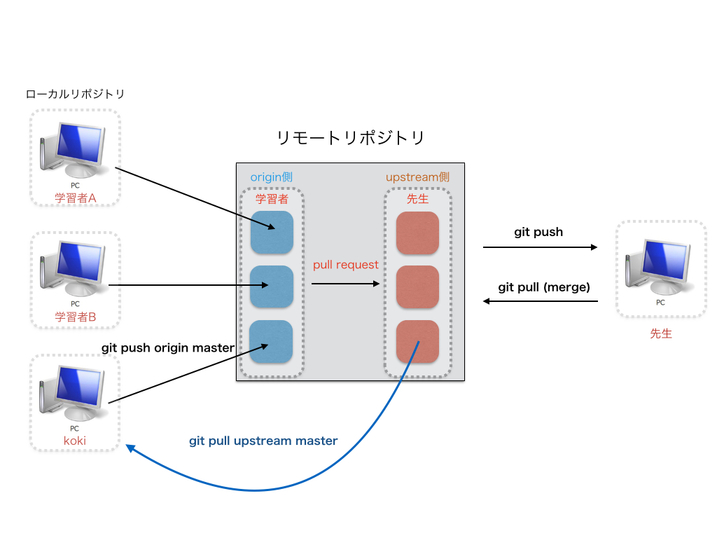
\includegraphics[width=12cm,bb= 0 0 737 553]{../figs/./ruby_novice.006.jpg}
\caption{Githubの仕組み.}
\label{default}\end{center}\end{figure}
ここからは,図1を参考にしながらGithubを利用した学習の流れを示す.

\subsubsection{進捗状況の報告}
まずは本研究での進捗状況の報告までの簡単な流れは以下の通りである.(git init, forkが済んでいると仮定)

\begin{enumerate}
\item ファイルを作成する.
\item git remote -v: originが自分のアドレスでupstreamが先生のアドレスであるか確かめる.
\item git add -A: 編集操作をlocalのrepositoryに登録.
\item git commit: ファイルの追加や変更の履歴をリポジトリに保存.
\item git push origin master: Githubのoriginへmasterをpush.
\item pull request: Githubで自分のサイトに載せた変更を,先生のサイトに変更希望として出す.コメント欄で変更詳細を伝えることが可能.
\end{enumerate}
基本的にローカルリポジトリで作業を行い,その作業内容をリモートポジトリ(Github)へプッシュする流れで行う.

\subsubsection{添削後の作業の流れ}
\begin{enumerate}
\item 先生がファイルを添削後,リモートリポジトリ(Github)にgit push.
\item git pull upstream master: 自分の開発中のファイルに反映.
\end{enumerate}
このサイクルを繰り返して,研究または,課題を進めていく.

それぞれの用語の説明は以下の通りである.

\begin{itemize}
\item リポジトリ:          ファイルやディレクトリの状態を保存する場所.
\item ローカルリポジトリ:  自分のマシン内にあるリポジトリ.
\item リモートリポジトリ:  サーバなどネットワーク上にあるリポジトリ.
\item コミット(commit):    ファイルの追加や変更の履歴をリポジトリに保存すること.
\item origin:              リポジトリの場所(URL)の別名.
\item master:              ブランチの名前.
\item プッシュ(push):      ファイルの追加や変更の履歴をリモートリポジトリにアップロードするための操作.
\end{itemize}
\subsection{コードテスト環境}
ruby\_noviceでは学習者自身で書いたコードを開発現場で使用されている一般的なテスト環境でテストする.本研究でモデルとしたテスト駆動開発ならびに比較検討したフレームワークを示す.

\subsubsection{TDD (Test Driven Development)}
2000年代初期に開発手法として確立された「テスト駆動開発」(Test Driven Development)は,その後10年もの間で普及が進み,今や珍しくない開発スタイルの1つとなっている.
国内でも「アジャイルアカデミー」「TDD Boot Camp」などによる推進・普及活動が各地で活発化し,認知が広がっている\cite{3}.

テスト駆動開発は,簡単に言うとプログラムを書く前にテストコードを書くということである.プログラムが完成した後にテストコードを書くのではなく,テストコードを先に書くことに大きな意味がある.
それは先に仕様を決め,テストコードを書くことによって自分が次にやることが明確になるためである.これにより作業効率も上がるメリットがある.最初にいきなりプログラムを書くと,整理されていないプログラムが出来てしまう.
しかしはじめにテストコードを書くことによって何をすべきか明確になるのでプログラムが書きやすくなる.他にTDDの目的としては,軽快なフィードバックの確保,きれいで動くコードの確保などによる開発の改善が挙げられる.
テスト駆動開発は, テストファーストによる追加・変更とリファクタリングによる設計改善という2つの活動で構成されている. 継続的にユニットテストを使って設計検討やチェック, リファクタリングを行うことにより, テスタビリティに優れバグの少ないソースコードを実現することが可能になる. 

\subsubsection{test::unitとは}
Ruby用のxUnit系の単体テストフレームワークである. Ruby1.8まではRuby本体に標準添付されていたが,Ruby1.9.1からはminitestというフレームワークが標準添付されている.
test-unitがRuby1.8に標準添付されていた頃はほとんど機能拡張などがされず,RSpecなど新しいテスティングフレームワークから見劣りするものとなっていた.
しかし,Ruby標準添付ではなく,1つのプロジェクトとして開発が進められるようになってからは活発に開発が進められている.Ruby本体のバージョンアップに関係なく新しいバージョンをリリースできるようになったことも開発が活発になった理由の一つである\cite{4}.

\subsubsection{arubaとは}
ArubaはCucumber,RSpec,Minitestのような人気のあるTDD/BDDフレームワークでコマンドラインアプリケーションのテストを簡単で楽しいものにする拡張である.
特徴としては以下の通りである\cite{5}.

\begin{itemize}
\item どんな言語で実装されたコマンドラインツールでもテスト可能.
\begin{itemize}
\item テスト自体はRubyで書くが,テスト対象は,PythonのCLIツールでもGolangのCLIツールでもよい.
\end{itemize}
\item ファイルシステムやプロセス環境をヘルパーによって操作できる.
\begin{itemize}
\item 例えば,readでファイルを読み込みできる.
\item 例えば,runで外部コマンドを実行し,その結果を have\_output matcher などで検証できる.
\end{itemize}
\item ファイルシステムやプロセス環境はテストのたびにリセットされるので,leaking stateがない.
\begin{itemize}
\item 例えばテスト中に作成されたファイルはテスト終了後には消えている.
\end{itemize}
\item コミュニティーサポートが手厚い.
\item ドキュメントにあるとおりに動作することが期待できる.
\end{itemize}

\section{結果と分析}
\subsection{ruby\_noviceの概要}
ruby\_noviceは,情報環境であるGitHubを利用しRuby初心者が文法だけでなく,Rubyプログラミングにおける振舞いを身につけるための支援ソフトを開発する.
またRubyプログラミングで重要となるテスト駆動をおこなえる環境を提供している.これにより,学習者自身が出力チェックできるようにしRubyプログラミングにおけるテスト実行に自然と慣れるような学習形態を目指している.

\subsection{ruby\_noviceの仕組み}
\begin{figure}[htbp]\begin{center}
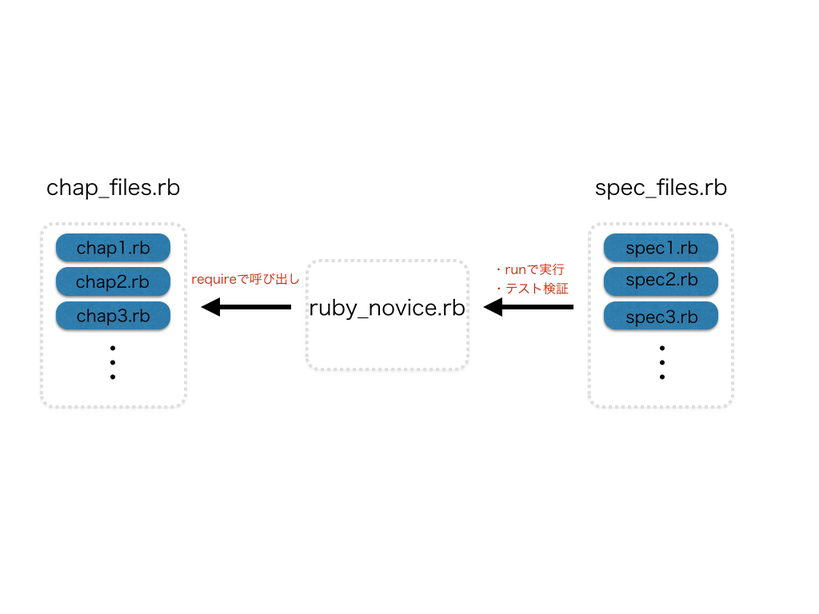
\includegraphics[width=6cm,bb=0 0 442 500]{../figs/./ruby_novice.001.jpg}
\caption{ruby\_noviceの構造.}
\label{default}\end{center}\end{figure}
ruby\_noviceの構造は,上記の図のように3つに分かれています.

\begin{itemize}
\item chap\_files.rb (chap1.rb, chap2.rb ...) : Text(たのしいRuby)のコードを書く部分.
\item ruby\_novice.rb :  chap\_files.rbを呼び出している.
\item spec\_files.rb  :  runで外部コマンドを入力して,出力結果 = 期待している値の検証.
\end{itemize}
テストコードが書いているspecファイルを各章ごとに分け,ruby\_novice.rbで呼び出すことにより,章ごとにテストを実行することを可能にした.

\begin{itemize}
\item 以下がruby\_novice.rbのコードの中身である. (たのしいRubyの1章のみ抜粋)
\end{itemize}\begin{quote}\begin{verbatim}
 #ruby_novice.rb
 
 $LOAD_PATH.unshift File.expand_path("../../lib/#{ENV['RUBYNOVICE_NAME']}", __FILE__)
 begin
   require "chap_files"
 rescue LoadError
   p "Load Error of ex_files in rubynovice.rb."
   p File.expand_path("../../lib/#{ENV['RUBYNOVICE_NAME']}", __FILE__)
   exit
 end
 
 require "ruby_novice/version"
 require 'thor'
 #require "code"                                                                                  
 
 module RubyNovice
   # Your code goes here...                                                                       
 
   class CLI < Thor
 #    class_option :help, type: :boolean, aliases: '-h', desc: 'help.'                            
 #    class_option :debug, type: :boolean, aliases: '-d', desc: 'debug mode'                      
 
 =begin                                                                                           
     desc 'hello', 'print hello'                     
     def hello                                                                                    
       my_hello                                                                                   
     end                                                                                          
 =end
 
     desc 'my_helloruby', 'print helloruby'
     def my_helloruby
       helloruby
     end
 
     desc 'my_puts_and_p', 'print puts_and_p'
     def my_puts_and_p
       puts_and_p
     end
 
     desc 'my_kiritsubo', 'print kiritsubo'
     def my_kiritsubo
       kiritsubo
     end
 
     desc 'my_area_volume', 'print area_volume'
     def my_area_volume
       area_volume
     end
 
     desc 'my_comment_sample', 'print comment_sample'
     def my_comment_sample
       comment_sample
     end
 
     desc 'my_greater_smaller', 'print greater_smaller'
     def my_greater_smaller
       greater_smaller
     end
 
     desc 'my_greater_smaller_else', 'print greater_smaller_else'
     def my_greater_smaller_else
       greater_smaller_else
     end
 
     desc 'version', 'version'
     def version
       puts RubyNovice::VERSION
     end
 
     private
 
     def output_error_if_debug_mode(e)
       return unless options[:debug]
       STDERR.puts(e.message)
       STDERR.puts(e.backtrace)
     end
   end
 end
\end{verbatim}\end{quote}
\begin{itemize}
\item 以下がchap1\_spec.rb のコードの中身である. (たのしいRubyの1章のみ抜粋)
\end{itemize}\begin{quote}\begin{verbatim}
 #spec_chap1.rb
 require 'spec_helper'
 
 RSpec.describe 'ruby_novie command', type: :aruba do
   context 'version option', type: :version do
     before(:each) { run('ruby_novice v') }
     it { expect(last_command_started).to be_successfully_executed }
     it { expect(last_command_started).to have_output("0.1.0") }
   end
 
   context 'help option', type: :help do
     expected = `bundle exec exe/ruby_novice help`
     before(:each) { run('ruby_novice help') }
     it { expect(last_command_started).to be_successfully_executed }
 #   it { expect(last_command_started).to have_output(expected) }               
   end
 
 =begin                                                                          
   context 'print hello', type: :hello do                                        
     before(:each) { run('ruby_novice hello') }                                  
     expected = "Hello."                                                         
     it { expect(last_command_started).to be_successfully_executed }             
     it { expect(last_command_started).to have_output(expected) }    
   end                                                                           
 =end 
 
   context 'helloruby', type: :helloruby do
     before(:each) { run('ruby_novice my_helloruby') }
     expected = "Hello, Ruby."
     it { expect(last_command_started).to be_successfully_executed }
     it { expect(last_command_started).to have_output(expected) }
   end
 
   context 'puts_and_p', type: :puts_and_p do
     before(:each) { run('ruby_novice my_puts_and_p') }
     expected = "Hello,\n\tRuby.\n\"Hello,\n\tRuby.\""
 
     it { expect(last_command_started).to be_successfully_executed }
     it { expect(last_command_started).to have_output(expected) }
   end
 
   context 'kiritsubo', type: :kiritsubo do
     before(:each) { run('ruby_novice my_kiritsubo') }
     expected = "いづれの御時にか女御更衣あまたさぶらいたまいけるなかに\nいとや\\
 むごとなき際にはあらぬがすぐれて時めきたまふありけり"
 
     it { expect(last_command_started).to be_successfully_executed }
     it { expect(last_command_started).to have_output(expected) }
   end
 
   context 'area_volume', type: :area_volume do
     before(:each) { run('ruby_novice my_area_volume') }
     expected = "表面積=2200\n体積=6000"
 
     it { expect(last_command_started).to be_successfully_executed }
     it { expect(last_command_started).to have_output(expected) }
   end
 
   context 'greater_smaller', type: :greater_smaller do
     before(:each) { run('ruby_novice my_greater_smaller') }
     expected = "greater"
 
     it { expect(last_command_started).to be_successfully_executed }
     it { expect(last_command_started).to have_output(expected) }
   end
 
 
   context 'greater_smaller_else', type: :greater_smaller_else do
     before(:each) { run('ruby_novice my_greater_smaller_else') }
     expected = "greater"
 
     it { expect(last_command_started).to be_successfully_executed }
     it { expect(last_command_started).to have_output(expected) }
   end
 end
 
\end{verbatim}\end{quote}
\subsection{ruby\_noviceの現状}
現状は,たのしいRubyの第1章~第7章までのテストコードを書き実装できる.
各章の概要は,以下の通りである.

\begin{itemize}
\item 第1章 (list1.1 ~ 1.7):  putsメソッドやpメソッド
\item 第3章 (list3.1 ~ 3.11): ファイルの読み込み
\item 第4章 (list4.1):        ローカル変数とグローバル変数
\item 第5章 (list5.1 ~ 5.5):  条件判断(if, unlessなど)
\item 第6章 (list6.1 ~ 6.13): 繰り返し(for,times,whileなど)
\item 第7章 (list7.1 ~ 7.4):  メソッド
\end{itemize}
(注意)

予約語(for,while)などは使えないため,以下の問題は名前を変更している.

\begin{itemize}
\item list5.3:  unless.rb → unless1.rbに変更.
\item list5.4:  case.rb → case1.rbに変更.
\item list6.4:  for.rb → for1.rbに変更.
\item list6.6:  while.rb → while11.rbに変更.
\item list6.9:  until.rb → until1.rbに変更.
\item list7.4:  myloop.rb → myloop1.rbに変更.
\end{itemize}
\subsection{ruby\_noviceの作業の流れ}
\begin{figure}[htbp]\begin{center}
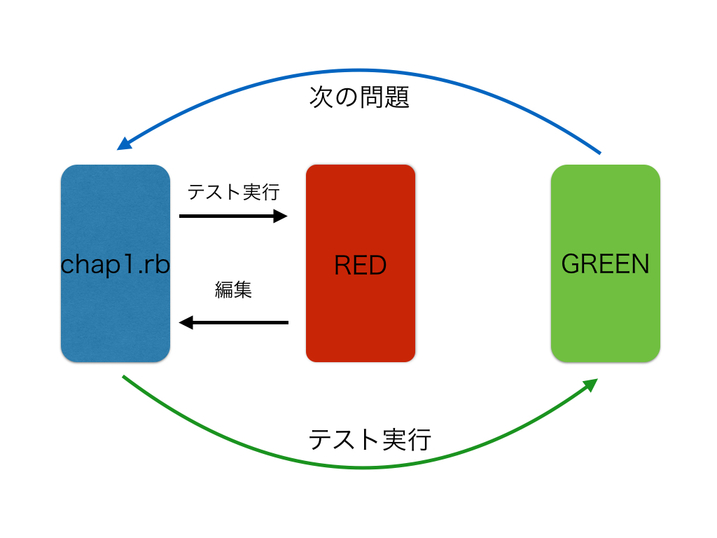
\includegraphics[width=6cm,bb=0 0 442 500]{../figs/./ruby_novice.003.jpg}
\caption{学習の流れ.}
\label{default}\end{center}\end{figure}
上記の図のようにRuby学習者はRed, Greenという作業サイクルを繰り返してプログラミングを進めていきます.

\begin{enumerate}
\item 作成したいプログラムの仕様を明確にする.
\item Red (テストに失敗)
\item Green(Redの状態ならば,編集しテストを成功させるコードを書く)
\item Greenになると次の問題に進む.
\end{enumerate}
Red,Greenという言葉は,TDDで多用されるテスティングフレームワークの多くがテスト失敗を赤色表示で,テスト成功を緑色表示で通知することに由来している.

\begin{figure}[htbp]\begin{center}
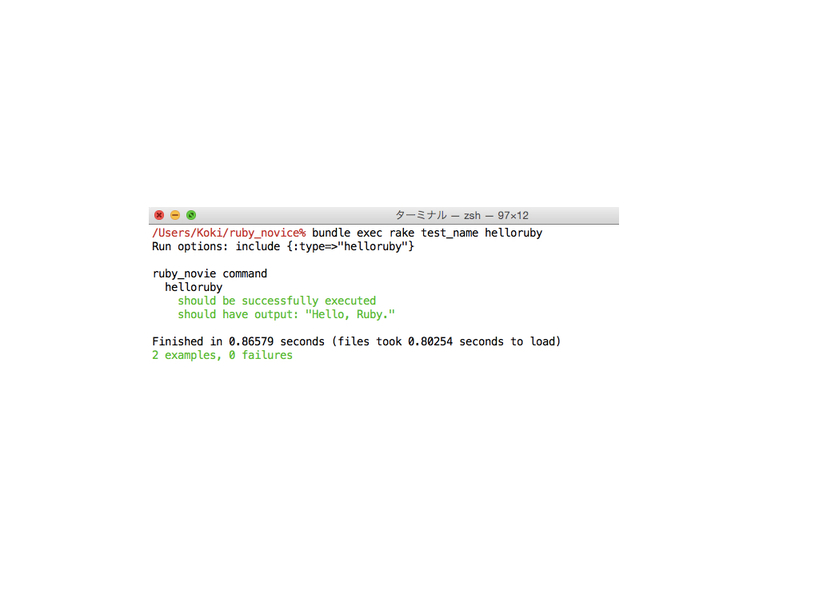
\includegraphics[width=6cm,bb=0 0 442 500]{../figs/./ruby_novice.004.jpg}
\caption{Greenの出力結果.}
\label{default}\end{center}\end{figure}
\begin{figure}[htbp]\begin{center}
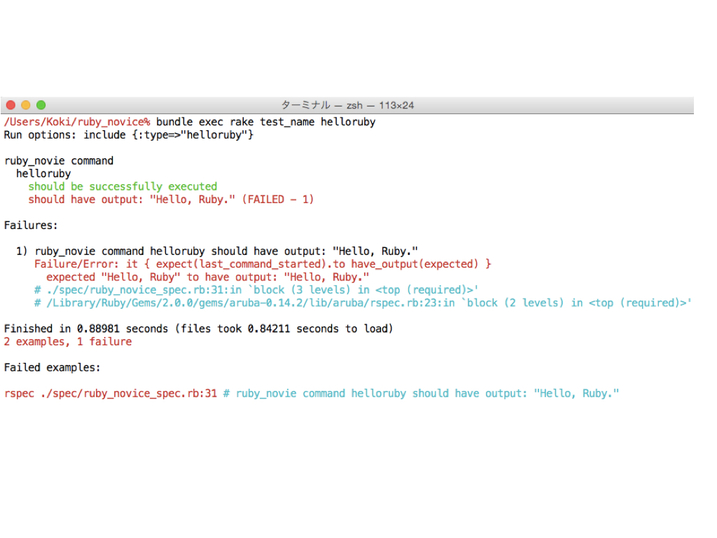
\includegraphics[width=6cm,bb=0 0 442 500]{../figs/./ruby_novice.005.jpg}
\caption{Redの出力結果.}
\label{default}\end{center}\end{figure}
\subsection{ruby\_noviceの使用法}
\begin{itemize}
\item 自分の好きな名前(koki)をつけたディレクトリを作成し,"./lib/koki/chap\_files.rb"を準備.
\end{itemize}
コード例
\begin{quote}\begin{verbatim}
  #/Users/Koki/ruby_novice% cat lib/koki/chap_files.rb
	
	 require "chap1"
  #require "chap3" 
  #require "chap4"
  #require "chap5"
  #require "chap6"
  #require "chap7"

	(注) # はコメントアウト.
\end{verbatim}\end{quote}
\begin{itemize}
\item chap1.rbというファイルを作り,そのファイルにたのしいRuby1章のlist(1.1~1.7)のコードを書いていく.
\end{itemize}
コード例 (たのしいRuby第1章)
\begin{quote}\begin{verbatim}
 #/Users/Koki/ruby_novice% cat lib/koki/chap1.rb
 
 def helloruby     
   print("Hello, Ruby.\n")
 end
 
 def puts_and_p
   puts "Hello,\n\tRuby."
   p "Hello,\n\tRuby."
 end
 
 def kiritsubo
   print "いづれの御時にか女御更衣あまたさぶらいたまいけるなかに\n"
   print "いとやむごとなき際にはあらぬがすぐれて時めきたまふありけり\n"
 end
 
 def area_volume
   x = 10
   y = 20
   z = 30
   area = (x*y + y*z + z*x) * 2
   volume = x * y * z
   print "表面積=", area, "\n"
   print "体積=", volume, "\n"
 end
 
 def comment_sample
 =begin                                                                          
   「たのしいRuby 第5版」サンプル                                               
    コメントの使い方の例                                                         
   2006/06/16 作成                                                              
    2006/07/01 一部コメントを追加                                                
    2015/10/01 第5版用に更新                                                    
 =end
 
   x = 10 # 縦                                                                   
   y = 20 # 縦                                                                   
   z = 30 # 高さ                                                                 
   # 表面積と体積を計算する                                                      
   area = (x*y + y*z + z*x) * 2
   volume = x * y * z
   # 出力する                                                                    
   print "表面積=", area, "\n"
   print "体積=", volume, "\n"
 end
 
 def greater_smaller
   a = 20
   if a >= 10 then
     print "greater\n"
   end
   if a <= 9 then
     print "smaller\n"
   end
 end
 
 def greater_smaller_else
   a = 20
   if a >= 10
     print "greater\n"
   else
     print "smaller\n"
   end
 end
 
\end{verbatim}\end{quote}
\begin{itemize}
\item rspecで,個人(koki)ごとのテストを実行するには, 環境変数RUBYNOVICE\_NAMEにディレクトリ名を入れる.
\begin{itemize}
\item (csh,tcsh)setenv RUBYNOVICE\_NAME koki
\item (bash,zsh)export RUBYNOVICE\_NAME=koki
\end{itemize}
\end{itemize}
\subsection{ruby\_noviceのコマンド}
\subsubsection{tagの表示の仕方}
\begin{itemize}
\item grep type spec/ruby\_novice\_spec.rb  で全てのcontextとtypeを表示.
\end{itemize}
typeは各章の各問題名の相当する.各問題ごとにテストする時に便利になる.
\begin{quote}\begin{verbatim}
  context 'version option', type: :version do
  context 'help option', type: :help do
  context 'print hello', type: :hello do
  context 'helloruby', type: :helloruby do
  context 'puts_and_p', type: :puts_and_p do
  context 'kiritsubo', type: :kiritsubo do
  context 'area_volume', type: :area_volume do
  context 'comment_sample', type: :comment_sample do
  context 'greater_smaller', type: :greater_smaller do
  context 'greater_smaller_else', type: :greater_smaller_else do
  context 'print_argv', type: :print_argv do
  context 'happy_birth', type: :happy_birth do
  context 'arg_arith', type: :arg_arith do
  context 'read_text', type: :read_text do
  context 'read_text_simple', type: :read_text_simple do
  context 'read_text_oneline', type: :read_text_oneline do
  context 'read_line', type: :read_line do
  context 'simple_grep', type: :simple_grep do
  context 'hello_ruby2', type: :hello_ruby2 do
  context 'use_grep', type: :use_grep do
  context 'scopetest', type: :scopetest do
  context 'ad2heisei', type: :ad2heisei do
  context 'if_elsif', type: :if_elsif do
  context 'unless1', type: :unless1 do
  context 'case1', type: :case1 do
  context 'case_class', type: :case_class do
  context 'times', type: :times do
  context 'times2', type: :times2 do
  context 'times3', type: :times3 do
  context 'for1', type: :for1 do
  context 'for_names', type: :for_names do
  context 'while1', type: :while1 do
  context 'while2', type: :while2 do
  context 'while3', type: :while3 do
  context 'until1', type: :until1 do
  context 'while_not', type: :while_not do
  context 'each_names', type: :each_names do
  context 'each', type: :each do
  context 'break_next', type: :break_next do
  context 'times_with_param', type: :times_with_param do
  context 'hello_with_name', type: :hello_with_name do
  context 'hello_with_default', type: :hello_with_default do
  context 'myloop1', type: :myloop1 do
\end{verbatim}\end{quote}
\subsection{全章のテストの仕方}
\begin{itemize}
\item bundle exec rspec
\end{itemize}
すべての章のテストを一括して実行できる.

\subsection{各章ごとのテストの仕方}
例: 1章(chap1)のテストをしたい時.

\begin{itemize}
\item bundle exec rspec spec/chap1\_spec.rb
\end{itemize}
\begin{itemize}
\item bundle exec rake chap 1
\end{itemize}
実行例
\begin{quote}\begin{verbatim}
 /Users/Koki/ruby_novice% bundle exec rake chap 1   
 
 ruby_novie command
   version option
     should be successfully executed
     should have output: "0.1.0"
   help option
     should be successfully executed
   helloruby
     should be successfully executed
     should have output: "Hello, Ruby."
   puts_and_p
     should be successfully executed
     should have output: "Hello,\n\tRuby.\n\"Hello,\n\tRuby.\""
   kiritsubo
     should be successfully executed
     should have output: "いづれの御時にか女御更衣あまたさぶらいたまいけるなかに\nいとやむごとなき際にはあらぬがすぐれて時めきたまふありけり"
   area_volume
     should be successfully executed
     should have output: "表面積=2200\n体積=6000"
   comment_sample
     should be successfully executed
     should have output: "表面積=2200\n体積=6000"
   greater_smaller
     should be successfully executed
     should have output: "greater"
   greater_smaller_else
     should be successfully executed
     should have output: "greater"
		 
 Finished in 7.61 seconds (files took 1.03 seconds to load)
 17 examples, 0 failures
\end{verbatim}\end{quote}
\subsubsection{各問題ごとのテストの仕方}
例: 各問題(helloruby)ごとにテストをしたい時.

\begin{itemize}
\item bundle exec rspec --tag type:helloruby spec/ruby\_novice\_spec.rb  (hellorubyは問題名)
\end{itemize}
\begin{itemize}
\item bundle exec rake test\_name helloruby
\end{itemize}
実行例
\begin{quote}\begin{verbatim}
/Users/Koki/ruby_novice% bundle exec rake test_name helloruby
Run options: include {:type=>"helloruby"}

ruby_novie command
  helloruby
    should be successfully executed
    should have output: "Hello, Ruby."
		 
Finished in 0.87128 seconds (files took 0.81684 seconds to load)
2 examples, 0 failures
\end{verbatim}\end{quote}
問題名は,上記のgrep type spec/ruby\_novice\_spec.rbで調べることができる.
typeが各問題の名前になる.またtextの問題名(例えばputs\_and\_p.rb)が,そのまま使えるのでテストも簡単にでき,問題名で中身のコードの内容も把握できる. 

\subsubsection{各問題ごとの実行結果の出力}
例: hellorubyの実行結果の出力

\begin{itemize}
\item bundle exec exe/ruby\_novice my\_helloruby
\end{itemize}
\begin{itemize}
\item bundle exec rake/output helloruby
\end{itemize}
実行例
\begin{lstlisting}[style=customRuby]
/Users/Koki/ruby_novice% bundle exec rake output helloruby
Hello, Ruby.
\end{lstlisting}

\section{考察}
\subsection{なぜaruba? (aruba vs test::unit)}
Cucumber,RSpec,Minitestのような人気のあるTDD/BDDフレームワークの中でもarubaを使用した理由は以下の通りである.
test:unitやarubaで書くとどうなるかを具体的に書いたコードを比べて示していきます.

\subsubsection{test::unitで書いたテストコード}
たのしいRubyのテキストに記載されている問題で比較していきたいと思います.
テキストの最初の問題は,Hello, Rubyを出力するプログラムです.
\begin{quote}\begin{verbatim}
print("Hello, Ruby.\n")
\end{verbatim}\end{quote}
まず,出力されるHello, Rubyをテストする場合のコードです.
\begin{lstlisting}[style=customRuby]
#helloruby.rb

def helloruby
  return "Hello, Ruby.\n"
end
\end{lstlisting}
\begin{itemize}
\item test::unitで書いたテストコード
\end{itemize}\begin{lstlisting}[style=customRuby]
require 'test/unit'
require './helloruby'

class Test_Sample < Test::Unit::TestCase
  def test_helloruby
    assert_equal("Hello, Ruby.\n",helloruby)
  end
end
print("Hello, ruby.\n")
\end{lstlisting}
テストコードの内容は以下の通りである.
Rubyで代表的なtest/unitというgemが提供されています.このプログラムの始め(require 'test/unit')で,test/unitを呼び出します.
Test::Unit::TestCaseを継承したクラスを用意し、test\_xxxというメソッドを定義するとそのメソッドがテストの実行対象になり,ここではそれぞれTest\_Sampleクラスとtest\_hellorubyメソッドがそれに該当します。
クラス名は大文字から始めるという規則がありますので注意してください.またメソッド名は,必ずtest\_ から始めなくてはいけません.ここでは単純にtest\_hellorubyとしています.実行してみると分かりますが,
test\_ がないとちゃんと動いてくれません.
テストコードは,assert\_equal(期待値),(実際の値)で実行結果を検証します.assert\_equalは,ふたつの引数をとり,第1引数は期待している結果で,第2引数はテストの対象です.両者が一致すればテストをパスし,一致しない場合はテストが失敗する.
補足ですが,test\_xxxというメソッドはクラス内に複数あっても構いません.また、1つのテストメソッド内にassert\_equalを複数書くのもOKです.
(とはいえ、原則として1テストメソッドにつき1アサーションとするのが望ましい)

このテストを実行すると以下のような出力になります.
\begin{lstlisting}[style=]
/Users/Koki/rubynovice/spec/test_unit/list1% ruby test_helloruby.rb 
Hello, ruby.
Loaded suite test_helloruby
Started.

Finished in 0.000982 seconds.

1 tests, 1 assertions, 0 failures, 0 errors, 0 pendings, 0 omissions, 0 notifications
100% passed

1018.33 tests/s, 1018.33 assertions/s
\end{lstlisting}
\subsubsection{test::unitでの問題点}
この場合だと初心者であるRubyの学習者がスクリプトとテストコードを同時に書かなければならない.学習者は,テストコードの書き方も学ぶ必要があるので,学習コストや間違えるリスクが大きくなる.
一番の問題点は,テキストを見ながら,その問題通りに書けないということです.先ほどの問題で説明すると,コードにreturnを付け加えなければならないことや,printメソッドはreturnできないので,テストするときは return "Hello, Ruby.\\n"と書き換えなければなりません.
このようにtest::unitだとメソッドを書き換えないといけないことや,printメソッドをreturnで返すことができないというデメリットがある.
そこでarubaはprintをそのまま出力できテストが可能である.学習者がtext(たのしいRuby)を見ながら書いていけるというメリットがあるので学習コストや間違えるリスクを削減できます.
実際にarubaで書いたコードを元にして具体的に示します.

\subsubsection{arubaで書いたテストコード}
先ほどと同じHello, Rubyを出力するプログラムをテストします.
\begin{quote}\begin{verbatim}
# code.rb

def helloruby    
  print("Hello, Ruby.\n")
end
\end{verbatim}\end{quote}\begin{quote}\begin{verbatim}
#ruby_novice.rb

require 'thor'                                                                         
require "code.rb"

module RubyNovice
  class CLI < Thor
    desc 'my_helloruby', 'print helloruby'
    def my_helloruby
      helloruby
    end
end
\end{verbatim}\end{quote}
require で,thorとcode.rbを呼び出しています.thorは,コマンドラインツールを作るためのgemです.
引数の受け渡しを簡潔に書くことができ,オプションのパースやUsage Message の表示など簡単に作成できます.

次にテストコードですが,arubaの場合printメソッドをreturnせずにそのままテストが可能になります.
下記がこの問題でのテストコードです.
\begin{lstlisting}[style=customRuby]
#ruby_novice_spec.rb

require 'spec_helper'

RSpec.describe 'ruby_novie command', type: :aruba do 
  context 'helloruby', type: :helloruby do
    before(:each) { run('ruby_novice my_helloruby') }
    expected = "Hello, Ruby."
    it { expect(last_command_started).to be_successfully_executed }
    it { expect(last_command_started).to have_output(expected) }
  end
end
\end{lstlisting}
テストコードの意味は次の通りです.
\begin{description}
\item[run('ruby\_novice my\_helloruby')]  ruby\_noviceのmy\_hellorubyを実行する.

\item[expected = "Hello, Ruby."]  期待している結果. test::unitでいう第1引数である.

\item[expect(last\_command\_started).to be\_successfully\_executed]  status 0 で終了していることを確認. このコードでエラーなく終了したことを確認する.

\item[expect(last\_command\_started).to have\_output(expected)]  出力がcontentsであることを確認,正規表現も使用可能である.このコードで期待値=実際の値であるかを検証します.両者が一致すればテストをパスし,一致しない場合はテストが失敗する.

\end{description}


\section{結論}
同じ課題に対して,実際にarubaでのテストコードとtest::unitでのテストコードを書き,具体的に出力結果やコードを比較した.これにより,双方の良い点や問題点を抽出することができた.当初の開発目的が,「Ruby初心者が文法だけでなく,Rubyプログラミングにおける振舞いを身につけるための支援ソフトの開発」であった.この目的に合致させるためにはarubaが最適であった.なぜarubaなのか以下に簡単にまとめてみた.
\begin{description}
\item[textに忠実なcode] test::unitだとテストコードとスクリプトを同時に書かないといけないので,Ruby初心者にしては学習コストや間違えるリスクが大きくなる.またtext(たのしいRuby)で書かれているコードにreturnを付け加えなければならないというデメリットがある.それに比べてarubaだとtext(たのしいRuby)のコードをそのまま写すだけでよく,そのコードを実行するだけでテストをすることができる.

\end{description}\begin{description}
\item[個別テストの可能性] テスト環境としては, 環境変数RUBYNOVICE\_NAMEにディレクトリ名を入れるだけで,個人ごとにテストすることができる.また章ごとにテストコードを書いているので,各章ごとや各問題ごとにテストができ,1問ずつ確認しながらコードを書いていくことが可能である.

\end{description}
今後の課題としては,現段階でtextの7章までしかテストコードを書けていないので引き続き書くことであったり,慣れてきたらtextの問題だけでなく応用の問題もテストコードを書いていくことである.また問題にClassがあるコード(8章以降)は, 今まで通りコードを写すだけではテストできないので別のTDDフレームワークでのテストと比較して考える.


\section{謝辞}
本研究を進めるにあたり,終始多大なるご指導,御鞭撻をいただいた西谷滋人教授に対し,深くご御礼申し上げます.
また,同研究室に所属する先輩方,同輩達からの様々な助力,知識の共有があり,本研究を大成することができました.
この場をお借りして心から深く感謝いたします.

\section{参考文献}
[1]「Ruby入門教育」,池本有里, 山本耕史, \verb|http://www.shikoku-u.ac.jp/education/docs/Ser.A%20No.37,Ser.B%20No.34-20.pdf.|

[2]「GitHub」,横田一輝, \verb|https://kotobank.jp/word/GitHub-1725201.|

[3]「テスト駆動開発/振る舞い駆動開発を始めるための基礎知識」,井芹洋輝, \verb|http://www.atmarkit.co.jp/ait/articles/1403/05/news035_3.html.|

[4]「test-unit - Ruby用単体テストフレームワーク」, \verb|https://test-unit.github.io/ja/|

[5]「QiitaAruba gemでCLIのテストを支援する」, tbpgr, \verb|http://qiita.com/tbpgr/items/41730edcdb07bb5b59ad.|


\end{document}
